\begin{frame}{Teoria de Tipos}
    % \begin{itemize}
    %     \item \citeonline{appel1998ssa} demonstra a equivalência entre código funcional e uma representação na forma SSA

    %     \item []

    %     \item [] \begin{figure}
    %         \centering
    %         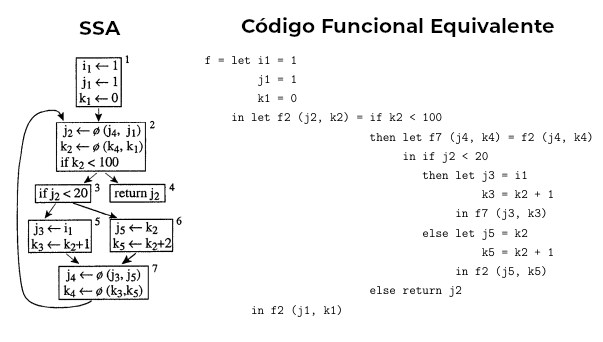
\includegraphics[width=.8\textwidth]{Figuras/ssa-funcional.png}
    %         \caption{Representações Equivalentes \cite{appel1998ssa}}
    %         \label{fig:conv1}
    %     \end{figure}
    % \end{itemize}
\end{frame}
